\documentclass[hyperref=unicode, aspectratio=169]{beamer}
\usepackage[utf8]{inputenc}
\usepackage[T2A]{fontenc}
\usepackage[russian]{babel}
\usepackage{csquotes}
\usepackage{tikzit}
\usepackage[justification=centering]{caption}
\usepackage{mathabx}
\usepackage{bookmark}
\usepackage{makecell}
\usepackage{listings}


\title[]{Построение многопроцессорного расписания с использованием жадных стратегий и ограниченного перебора}
\usetheme{Madrid}
\author[]{Савицкий Илья\\Научный руководитель: к.т.н. доцент Костенко Валерий Алексеевич}
% \medskip
% \texttt{Научный руководитель: к.т.н. доцент Костенко Валерий Алексеевич}
\date{26 мая 2022 г.}
\logo{
\includegraphics[width=1.5cm]{imgs/asvk-logo.png}}


\definecolor{ASVKaccent}{rgb}{0.20392,0.02745,0.34509}
\usecolortheme[named=ASVKaccent]{structure}

\input{block-schemas.tikzstyles}

\begin{document}
\begin{frame}
    \titlepage
\end{frame}

\section{Цель и задачи курсовой работы}
\begin{frame}
    \frametitle{Цели и задачи курсовой}
    Целью этой курсовой работы является разработка алгоритма построения многопроцессорного расписания с дополниьельными ограничениями на основе комбинации жадных стратегий и ограниченного перебора. 

    Для достижения указанной цели требуется:
    \begin{enumerate}
        \item Провести обзор алгоритмов построения списочных расписаний с целью выявления жадных критериев и схем ограниченного перебора которые могут быть модифицированы для решения данной задачи.
        \item Разработать и реализовать алгоритм.
        \item Провести исследование свойств алгоритма.
    \end{enumerate}
\end{frame}

\section{Описание прикладной задачи}
\begin{frame}
    \frametitle{Постановка задачи}
    \begin{columns}
        \begin{column}{0.60\textwidth}
            Дано:
            \begin{enumerate}
                \item Ориентированный граф работ $G$ без циклов, в котором дуги - зависимости по данным, а вершины - задания. Вершин $n$, дуг $m$
                \item Вычислительная система, состоящая из $p$ различных процессоров
                \item Матрица $C_{ij}$ длительности выполнения работ на процессорах, $i=1 \dots n, j=1 \dots p$. Каждая строка этой матрицы - длины выполнения $n$-й задачи на $p$ процессорах. 
                \item Матрица $D_{kl}$ передач данных между процессорами, $k=1 \dots p, l = 1 \dots p, D_{kk} = 0$. $D_{ij}$-й элемент этой матрицы - время пеердачи данных между процессорами $i$ и $j$.
            \end{enumerate}
        \end{column}
        \begin{column}{0.40\textwidth}
            \begin{figure}
                \ctikzfig{graph_schema}
                \captionsetup{labelformat=empty}
                \caption{Граф потока данных}
            \end{figure}
        \end{column}
    \end{columns}
\end{frame}

\begin{frame}
    \frametitle{Расписание}
    Расписание программы определено, если
    \begin{enumerate}
        \item Множества процессор и работ
        \item Привязка
        \item Порядок
    \end{enumerate}
    \par
    Привязка - всюду определенная на множестве работ функция, которая задает распределение работ по процессорам
    \par
    Порядок задает ограничения на последовательность выполнения работ и является отношением частичного порядка, удовлетворяющим условиям ацикличности и транзитивности. Отношение порядка на множестве работ, распределенных на \\один процессор, является отношением полного порядка.
\end{frame}

\begin{frame}
    \frametitle{Графическая форма представления расписания}
    \begin{figure}
        \small
        \ctikzfig{figures/schedule-graphical-form}
        \captionsetup{labelformat=empty}
        \caption{\small Графическая форма представления расписания}
    \end{figure}
    Графическая форма представления расписания $\Leftrightarrow$ Временная диаграмма
\end{frame}

\begin{frame}
    \frametitle{Постановка задачи}
    \begin{columns}
        \begin{column}{0.7\textwidth}
            Требуется:
            \begin{enumerate}
                \item Построить расписание $HP$, то есть для $i$-й работы определить время начала ее выполнения $s_i$ и процессор $p_i$ на которм она будет выполняться
                \item Минимизируемый критерий: время завершения выполнения расписания
                \item Дополнительные ограничения
            \end{enumerate}
        \end{column}
        \begin{column}{0.3\textwidth}
            \begin{figure}
                \tiny
                \ctikzfig{figures/schedule-time-diagram}
                \captionsetup{labelformat=empty}
                \caption{\small Представление расписания в виде временной диаграммы}
            \end{figure}
        \end{column}
    \end{columns}
\end{frame}

\begin{frame}
    \frametitle{Модель расписания}
    Множество корректных расписаний $HP$ задается набором ограничений:
    \begin{itemize}
        \item В расписании не допустимы прерывания
        \item Интервалы выполнения заявок не пересекаются
        \item Каждая работа назначена на процессор
        \item Любую работу обслуживает один процессор
        \item Частичный порядок, заданный графом зависимостей $G$, сохранен в $HP: G \subset G_{HP}^T$, где $G_{HP}^T$ - транзитивное замыкание отношения $G_{HP}$
    \end{itemize}
\end{frame}

\begin{frame}
    \frametitle{Постановки задачи}
    \begin{enumerate}
        \item Задача с однородными процессорами (длительность выполнения работы не зависит от того, на каком процессоре она выполняется) и дополнительными ограничениями на количество передач:
              \begin{itemize}
                  \item $CR = \frac{m_{ip}}{m}$, где $m_{ip}$ - количество передач данных между работами на каждый процессор
                        \vspace{5pt}
                  \item $CR2 = \frac{m_{2edg}}{m}$, где $m_{2edg}$ - количество дуг, начальный и конечный узлы которых назначены на процессоры, не соединенных напрямую
              \end{itemize}
        \item Задача с однородными процессорами и дополнительным ограничением сбалансированности распределения работ:
              \begin{itemize}
                  \item $BF = \left( \frac{a_{max} \cdot p}{n} \right) - 1$, где $a_{max}$ - наибольшее, по всем процессорам, количество работ на процессоре
              \end{itemize}
        \item Задача с неоднородными процессорами, но без дополнительных \\ограничений на расписание
    \end{enumerate}
\end{frame}


\section{Выводы по обзору}
\begin{frame}
    \frametitle{Обзор существующих алгоритмов}
    {
        \small
        \begin{tabular}{ c | c | c | c  }
            \makecell{Название          \\алгоритма} & Рандомизированность & Итерационный & \makecell{Возможность \\ масштабирования} \\
            \hline
            \makecell{Генетические      \\алгоритмы} & Рандомный & Итерационный & +/- \\
            \makecell{Алгоритм имитации \\отжига} & Рандомный & Итерационный & + \\
            \makecell{Муравьиные        \\алгоритмы} & Рандомный & Итерационный & - \\
            \makecell{Жадные стратегии  \\и ограниченный перебор} & Детерминированный & Конструктивный & + \\
        \end{tabular}
    }
\end{frame}

\section{Описание предложенного алгоритма}
\subsection{Дополнительные обозначения}
\begin{enumerate}
    \item $D= \left( d_1, d_2, \dots, d_l \right)$, где $l$ - количество вершин, доступных для добавления(т.е. у которых нет предшественников в графе $G$) - множество вершин, доступных для добавления в расписание.
    \item $k$ - вектор длин критических путей от ``головной'' вершины до каждой вершины графа.
    \item $\left( s_i, p_i \right)$ - достаточное количество информации для размещения работы в расписании.
\end{enumerate}
Жадные критерии
\begin{enumerate}
    \item $GR1$ - критерий, используемый в выборе работы на постановку
    \item $GR2$ - критерий, используемый в выборе места постановки работы
\end{enumerate}
Процедуры ограниченного перебора
\begin{enumerate}
    \item $H1$ - процедура перебора для создания места для постановки работы. Минимизируемый критерий - $s_i$
    \item $H2$ - процедура перебора для приближения времени старта работы к длине критического пути до нее. Минимизируемый критерий - $\sum s_k$, где $s_k$ - времена начала $k$ последних добавленных работ.
\end{enumerate}

\subsection{Словесное описание алгоритма}
\begin{enumerate}
    \item Сформировать множество вершин, у которых нет предшественников. Множество $D = \left( d_1, d_2 \dots d_i \right)$ где $d_i$ – номер работы, доступной для добавления в расписание (т.е. у которой нет предшественников в исходном графе)
    \item В случае, если в множестве $D$ одна вершина – обозначим ее за $d$, в противном случае – создадим фиктивную вершину с нулевой длительностью, у которой все потомки будут из множества $D$, и обозначим ее за $d$
    \item Зададим вектор $k$ – вектор длин критических путей до вершин от $d$. При помощи алгоритма Дейкстры этот вектор заполняется значениями $k_i$, где $i$ – номер вершины. Поскольку алгоритм Дейкстры работает со взвешенными графами, каждое ребро получает вес минимального времени работы на вычислительной системе вершины, из которой исходит
    \item \label{itm:calcD} По жадному критерию $GC1$ выбирается работа из множества $D$ для размещения в расписании. Пусть выбранная работа – $d_i$
    \item Производится пробное размещение работы $d$ в расписании с учетом жадного критерия $GC2$ и дополнительных ограничений. В случае, если не получилось найти подходящее место для работы – запускается процедура ограниченного перебора $H1$. Становится известно $s$ – время старта работы и $p$ – процессор, на котором работа выполняется.
    \item Если $s_i$ больше длины критического пути (с точностью до $\Delta$, где $\Delta$ – параметр алгоритма), то вызывается процедура ограниченного перебора $H2$. Если работу разместить не удалось – завершить алгоритм. Если $s_i$ не превосходит длину критического пути (с точностью $\Delta$), то работа размещается в расписании.
    \item $d_i$ удаляется из списка размещенных работ и в графе $G$ удаляется соответствующая вершина и все дуги, исходящие из нее.
    \item Обновляется множество $D$. Если $D$ не пустое, то алгоритм переходит на пункт \ref{itm:calcD}.
\end{enumerate}
\subsubsection*{Жадный критерий выбора работы $GC1$}
\begin{itemize}
    \item Максимальное количество потомков у работы
\end{itemize}
Такой выбор работы позволяет открыть максимально возможное количество кандидатов на следующую постановку задачи в расписание, а значит с минимальной вероятностью закрывает путь к оптимальному решению.
\subsubsection*{Жадный критерий выбора места работы в расписании $GC2$}
\begin{itemize}
    \item Скорейшее завершение частично построенного расписания
\end{itemize}
\subsubsection*{Выбор места работы в расписании}
\begin{itemize}
    \item Взвешенная сумма.
          \begin{gather*}
              crit = C_1 \cdot GC2 + C_2 \cdot CR + C_3 \cdot CR2
          \end{gather*}
          где $C_1$, $C_2$ и $C_3$ - параметры алгоритма. Работа размещается на место с наибольшим значением параметра $crit$.
    \item Допускная система выбора
          \begin{enumerate}
              \item Список мест размещения работ ранжируется по $GC2$, после чего отсекаются верхние $n\%$ работ, где $n$ - параметр алгоритма
              \item Такие же действия повторяются для каждого дополнительного ограничения
              \item В конечном списке выбрать место по жадному критерию
          \end{enumerate}
\end{itemize}
При ранжировании задач по взвешенной сумме возможна ситуация, при которой будет выбрано место которое хорошо проходит по одному критерию, но очень плохо по другому и тогда расписание будет строиться в направлении ложного минимума. Поэтому в программной реализации было выбрано использование допускной системы выбора.
\subsubsection*{Ограниченный перебор}
После неудачной пробной постановки работы в расписание алгоритм создает набор $K = \left( k_1, k_2, \dots, k_t \right)$, состоящий из $t$ последних добавленных работ ($t$ – параметр алгоритма). Далее, процедурой полного перебора пробуются различные расписания до тех пор, пока не получится расписание, удовлетворяющее критерию критичности пути до последней поставленной работы и удовлетворяющее дополнительным ограничениям.
\subsubsection*{Расчет времени начала работы}
Для того, чтобы рассчитать время начала  для конкретной работы на процессоре $p$ требуется:
\begin{enumerate}
    \item Вычислить вектор $PJ_{k=1}^L$, где $L$ – количество предшественников у работы. Элементами этого вектора будут являться суммы вида $s_k + C_{kr} + D_{rj}$, где $r$ – номер процессора, на котором размещен предшественник.
    \item Максимумом этого вектора и будет являться первое доступное начало выполнения работы на данном процессоре. $n_j=\max{PJ}$
\end{enumerate}

\subsection{Блок-схема алгоритма}
{\small
    \tikzfig{main-block-schema}
}

\section{Программная реализация}
\begin{frame}
    \frametitle{Программная реализация}
    Алгоритм реализован на языке \lstinline{C++} с помощюь фреймворка \lstinline{boost}.

    Проект обладает следующей структурой:
    \begin{enumerate}
        \item \lstinline{logging} - функции настройки логирования для проекта. Реализовано на основе \lstinline{Boost::log}
        \item \lstinline{schedule} - модуль для работы с графом входных данных и матрицами $C$ и $D$, подаваемыми на вход. Реализован на основе \lstinline{Boost::graph} и \lstinline{Boost::uBLAS}.
        \item \lstinline{time_schedule} - модуль для работы с временной диаграммой.
        \item \lstinline{main.cpp} - \lstinline{main()} программы. Основной алгоритм реализован тут. Разбор аргументов основан на \lstinline{Boost::program_options}.
        \item \lstinline{Doxyfile} - файл с настройками \lstinline{Doxygen}.
    \end{enumerate}

    Для сборки проекта используется \lstinline{CMake}.
\end{frame}

\section{Результаты исследования}
\begin{frame}
    \frametitle{Точность полученного расписания}
    \begin{columns}
        \begin{column}{0.5\textwidth}
            \begin{figure}
                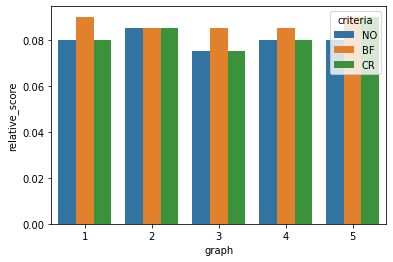
\includegraphics[width=\textwidth]{imgs/relative_score.png}
            \end{figure}
        \end{column}
        \begin{column}{0.5\textwidth}
            \begin{table}
                \caption*{Наборы исходных данных, используемых в тестировании}
                \begin{tabular}{c | c | c | c}
                    Граф & Вершин & Процессоров & Передач \\
                    \hline
                    1    & 126    & 4           & 716     \\
                    2    & 417    & 8           & 2367    \\
                    3    & 408    & 8           & 8763    \\
                    4    & 296    & 8           & 395     \\
                    5    & 93     & 4           & 92      \\
                \end{tabular}
            \end{table}
            % \begin{enumerate}
            %     \item 126 вершин, 4 процессора, 716 передач данных
            %     \item 417 вершин, 8 процессоров, 2367 передач данных
            %     \item 408 вершин, 8 процессоров, 8763 передач данных
            %     \item 396 вершин, 8 процессоров, 395 передачи данных
            %     \item 93 вершины, 4 процессора, 92 передачи данных
            % \end{enumerate}
        \end{column}
    \end{columns}

    \begin{equation*}
        relative\_score = \frac{\text{время полученного расписания}}{\text{время оптимального расписания}} - 1
    \end{equation*}
\end{frame}

\begin{frame}
    \frametitle{Время выполнения программы}
    \begin{figure}
        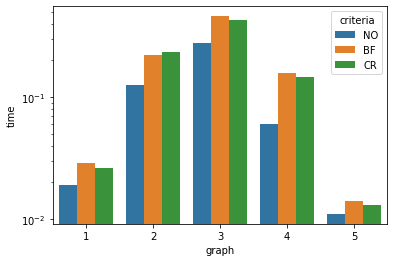
\includegraphics[width=0.7\textwidth]{imgs/times.png}
    \end{figure}
\end{frame}

\section{Полученные рещультаты}
\begin{frame}
    \frametitle{Текущие результаты}
    Реализвано:
    \begin{enumerate}
        \item Проведен обзор алгоритмов построения списочных расписаний. Цель обзора; выявление жадных критериев и схем ограниченного перебора которые могут быть модифицированы для решения данной задачи.
        \item Разработан алгоритм, основанный на сочетании жадных стратегий и ограниченного перебора.
        \item Реализован алгоритм.
        \item Подобраны оптимальные параметры алгоритма.
        \item Проведено исследование свойств алгоритма.
    \end{enumerate}
\end{frame}

\end{document}